\teaser{
	\centering
	\vspace{-1cm}
	\addtolength{\tabcolsep}{-4.5pt}
	\newlength{\insetLen}
	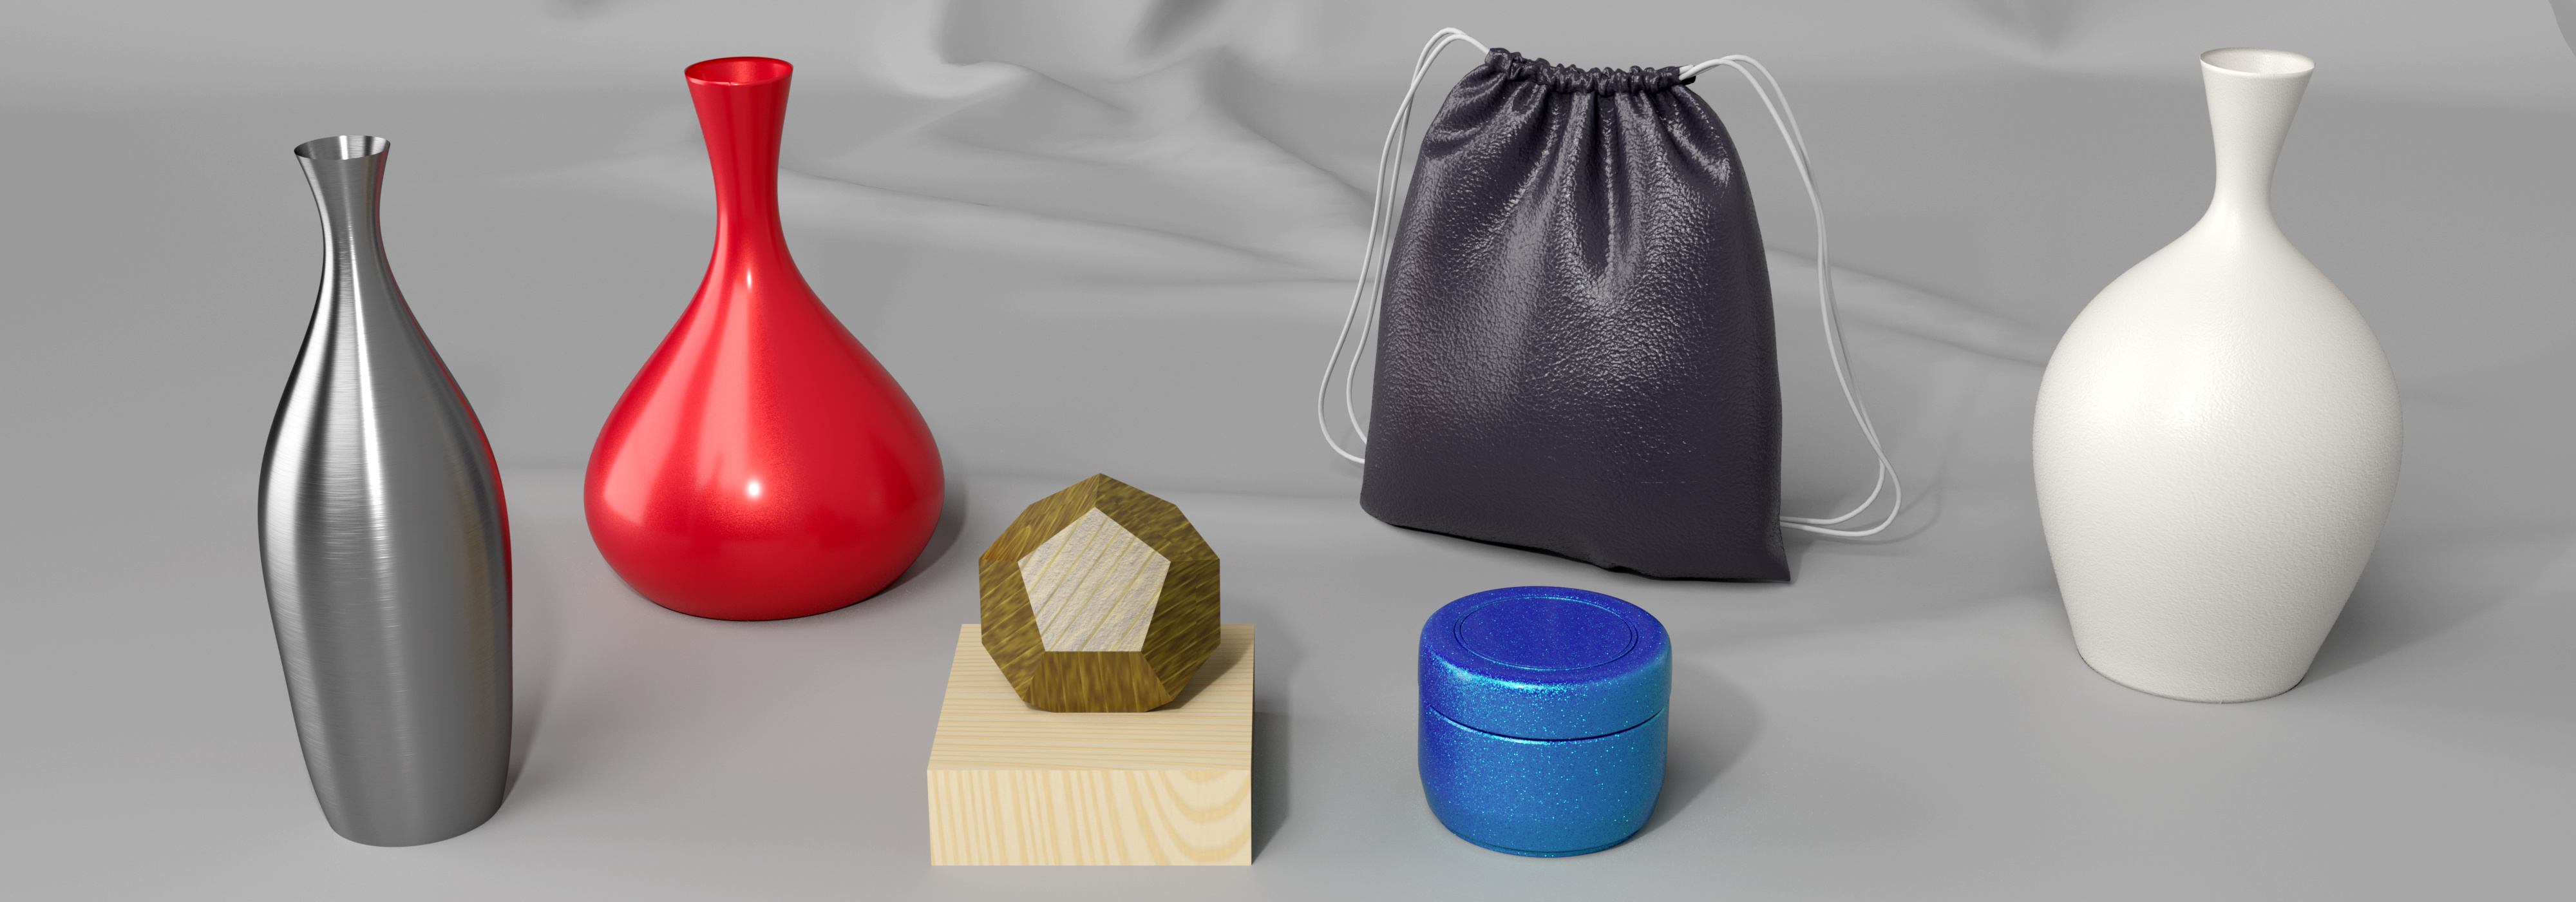
\includegraphics[width=\textwidth]{img/teaser.jpg}\\[3pt]
	\setlength{\insetLen}{0.134\textwidth}
	\begin{tabular}{cccccccc}
		\raisebox{7pt}{\rotatebox{90}{\small \bfseries Input}} &
		\adjincludegraphics[width=\insetLen,trim={0 {.2\height} 0 {.2\height}},clip]{real/metal_1/target.jpg} &
		\adjincludegraphics[width=\insetLen,trim={0 {.2\height} 0 {.2\height}},clip]{real/flake_2/target.jpg} &
		\adjincludegraphics[width=\insetLen,trim={0 {.2\height} 0 {.2\height}},clip]{real/wood_2/target.jpg} &
		\adjincludegraphics[width=\insetLen,trim={0 {.2\height} 0 {.2\height}},clip]{real/wood_3/target.jpg} &
		\adjincludegraphics[width=\insetLen,trim={0 {.2\height} 0 {.2\height}},clip]{synth/flake_1/target.jpg} &
		\adjincludegraphics[width=\insetLen,trim={0 {.2\height} 0 {.2\height}},clip]{real/leather_1/target.jpg} &
		\adjincludegraphics[width=\insetLen,trim={0 {.2\height} 0 {.2\height}},clip]{real/bump_2/target.jpg}
		\\
		\raisebox{3pt}{\rotatebox{90}{\small \bfseries Rendered}} &
		\adjincludegraphics[width=\insetLen,trim={0 {.2\height} 0 {.2\height}},clip]{real/metal_1/good1.jpg} &
		\adjincludegraphics[width=\insetLen,trim={0 {.2\height} 0 {.2\height}},clip]{real/flake_2/good1.jpg} &
		\adjincludegraphics[width=\insetLen,trim={0 {.2\height} 0 {.2\height}},clip]{real/wood_2/good1.jpg} &
		\adjincludegraphics[width=\insetLen,trim={0 {.2\height} 0 {.2\height}},clip]{real/wood_3/good1.jpg} &
		\adjincludegraphics[width=\insetLen,trim={0 {.2\height} 0 {.2\height}},clip]{synth/flake_1/good1.jpg} &
		\adjincludegraphics[width=\insetLen,trim={0 {.2\height} 0 {.2\height}},clip]{real/leather_1/good1.jpg} &
		\adjincludegraphics[width=\insetLen,trim={0 {.2\height} 0 {.2\height}},clip]{real/bump_2/good1.jpg}
	\end{tabular}
	\captionsetup{labelfont=bf,textfont=it}
	\caption{
			A scene rendered with material parameters estimated using our method: bumpy dielectrics, leather, plaster, wood, brushed metal, and metallic paint. The insets show a few examples of the input (target) images, and renderings produced using our procedural models with parameters found by Bayesian posterior sampling.
		\vspace{3mm}
 	}
	\label{fig:teaser}
}
